% concatenated from heinz_meanv1.tex
%% 
%% Copyright 2007-2020 Elsevier Ltd
%% 
%% This file is part of the 'Elsarticle Bundle'.
%% ---------------------------------------------
%% 
%% It may be distributed under the conditions of the LaTeX Project Public
%% License, either version 1.2 of this license or (at your option) any
%% later version.  The latest version of this license is in
%%    http://www.latex-project.org/lppl.txt
%% and version 1.2 or later is part of all distributions of LaTeX
%% version 1999/12/01 or later.
%% 
%% The list of all files belonging to the 'Elsarticle Bundle' is
%% given in the file `manifest.txt'.
%% 

%% Template article for Elsevier's document class `elsarticle'
%% with numbered style bibliographic references
%% SP 2008/03/01
%%
%% 
%%
%% $Id: elsarticle-template-num.tex 190 2020-11-23 11:12:32Z rishi $
%%
%%
\documentclass[preprint,12pt]{elsarticle}

%% Use the option review to obtain double line spacing
%% \documentclass[authoryear,preprint,review,12pt]{elsarticle}

%% Use the options 1p,twocolumn; 3p; 3p,twocolumn; 5p; or 5p,twocolumn
%% for a journal layout:
%% \documentclass[final,1p,times]{elsarticle}
%% \documentclass[final,1p,times,twocolumn]{elsarticle}
%% \documentclass[final,3p,times]{elsarticle}
%% \documentclass[final,3p,times,twocolumn]{elsarticle}
%% \documentclass[final,5p,times]{elsarticle}
%% \documentclass[final,5p,times,twocolumn]{elsarticle}

%% For including figures, graphicx.sty has been loaded in
%% elsarticle.cls. If you prefer to use the old commands
%% please give \usepackage{epsfig}

%% The amssymb package provides various useful mathematical symbols
\usepackage{amssymb}
\usepackage{enumerate}
\usepackage{csquotes}
%\usepackage{backref}
%\newtheorem{xca}[theorem]{Exercise}
%\newtheorem{problem}[theorem]{Problem}
%\theoremstyle{remark}
%\newtheorem{rem}[theorem]{Remark}
\usepackage{mathtools}
\usepackage{amssymb}
 \newtheorem{thm}{Theorem}[section]
 \newtheorem{theorem}{Theorem}[section]
 \newtheorem{conclusion}{Conclusion}
 \newtheorem{cor}[thm]{Corollary}
 \newtheorem{corollary}[thm]{Corollary}
\newproof{proof}{\textbf{Proof}}
 \newtheorem{lem}[thm]{Lemma}
 \newtheorem{lemma}[thm]{Lemma}
 \newtheorem{prop}[thm]{Proposition}
 \newtheorem{proposition}[thm]{Proposition}
 \newtheorem{defn}[thm]{Definition}
 \newtheorem{definition}[thm]{Definition}
 \newtheorem{rem}[thm]{Remark}
 \newtheorem{remark}[thm]{Remark}
 \newtheorem{example}{Example}
 \numberwithin{equation}{section}
\usepackage{epsfig,subfigure}
\usepackage{epstopdf}
\usepackage{geometry}
\usepackage{graphicx}
\usepackage{graphics}
\usepackage{subfigure}
\usepackage{tikz}
\usepackage{hyperref}
%% The amsthm package provides extended theorem environments
%% \usepackage{amsthm}

%% The lineno packages adds line numbers. Start line numbering with
%% \begin{linenumbers}, end it with \end{linenumbers}. Or switch it on
%% for the whole article with \linenumbers.
%% \usepackage{lineno}

%\journal{Nuclear Physics B}

\begin{document}

\begin{frontmatter}

%% Title, authors and addresses

%% use the tnoteref command within \title for footnotes;
%% use the tnotetext command for theassociated footnote;
%% use the fnref command within \author or \address for footnotes;
%% use the fntext command for theassociated footnote;
%% use the corref command within \author for corresponding author footnotes;
%% use the cortext command for theassociated footnote;
%% use the ead command for the email address,
%% and the form \ead[url] for the home page:
%% \title{Title\tnoteref{label1}}
%% \tnotetext[label1]{}
%% \author{Name\corref{cor1}\fnref{label2}}
%% \ead{email address}
%% \ead[url]{home page}
%% \fntext[label2]{}
%% \cortext[cor1]{}
%% \affiliation{organization={},
%%             addressline={},
%%             city={},
%%             postcode={},
%%             state={},
%%             country={}}
%% \fntext[label3]{}

\title{Some inequalities related to Heinz mean constant with Birkhoff orthogonality}

%% use optional labels to link authors explicitly to addresses:
%% \author[label1,label2]{}
%% \affiliation[label1]{organization={},
%%             addressline={},
%%             city={},
%%             postcode={},
%%             state={},
%%             country={}}
%%
%% \affiliation[label2]{organization={},
%%             addressline={},
%%             city={},
%%             postcode={},
%%             state={},
%%             country={}}

\author{Kallal Pal} %% 
\author{Sumit Chandok\corref{cor}}
\cortext[cor]{Corrosponding author.}\ead{sumit.chandok@thapar.edu}
%% Author affiliation
\affiliation{organization={Department of Mathematics,\\ Thapar Institute of Engineering and Technology},%Department and Organization
            city={Patiala},
            postcode={147004}, 
            state={Punjab},
            country={India}}
\begin{abstract}
%% Text of abstract
Motivated by the work of  Baronti et al. [J. Math. Anal. Appl. 252(2000)
124-146], where they defined the supremum of an arithmetic mean of the side lengths of a triangle, summing antipodal points on the unit sphere, we introduce a new geometric constant for Banach spaces, utilizing the Heinz means that interpolate between the geometric and arithmetic means associated with Birkhoff orthogonality. We discuss the bounds in Banach spaces and find the values of constant in Hilbert spaces.  We obtain the characterization of uniformly non-square spaces. We investigate the correlation between our notion of the Heinz mean constant and other well-known terms, viz., the modulus of convexity, modulus of smoothness, and rectangular constant.
Furthermore, we also
 give a characterization of the Radon plane with an affine regular hexagonal unit sphere.
\end{abstract}

%%Graphical abstract
% \begin{graphicalabstract}
% %\includegraphics{grabs}
% \end{graphicalabstract}

%%Research highlights
% \begin{highlights}
% \item Research highlight 1
% \item Research highlight 2
% \end{highlights}

\begin{keyword}
Geometric constant, Birkhoff orthogonality, Banach space. 
%% keywords here, in the form: keyword \sep keyword

%% PACS codes here, in the form: \PACS code \sep code

%% MSC codes here, in the form: \MSC code \sep code
%% or \MSC[2008] code \sep code (2000 is the default)

\end{keyword}

\end{frontmatter}

%% \linenumbers

%% main text
\section{Introduction}
The quantitative framework for analyzing the geometry of Banach spaces is provided by the study of geometric constants, which is essential for addressing numerous problems in functional analysis. In addition to describing the basic structure of normed spaces, these constants show complex relationships that are both mathematically beautiful and novel. Using specified constants to study abstract properties of Banach spaces has led to impressive characterizations of inner product spaces and many fascinating open topics in modern mathematics.

Banach spaces do not accept a single or canonical notion of orthogonality, in contrast to Euclidean geometry; instead, several ideas of orthogonality exist, none of which is necessarily equivalent. Birkhoff \cite{birkhoff1935orthogonality} was the first to introduce a fundamental notion of orthogonality in 1935, and James \cite{james1947orthogonality} suggested isosceles orthogonality in 1947. 
These developments have stimulated extensive research on the interaction between generalized orthogonality and geometric constants, emphasizing the complexity of Banach space theory and its importance in both pure and applied mathematics.

Clarkson introduced the modulus of convexity \cite{clarkson1936uniformly} which controls quantitatively how far the midpoint of two distant unit vectors is from the unit sphere. If the modulus of convexity is non-negative, then the Banach space is uniformly convex. Banas \cite{banas1986moduli} introduced the modulus of smoothness, which measures how rounded the unit ball is inward (quantifying uniform smoothness).
In 1990, Gao and Lau \cite{gao1990geometry} defined the James constant, or
the non-square constant, to characterize uniformly non-square. 
 Recently, Baronti and Papini \cite{papini2022parameters} discussed James constant under the restriction of Birkhoff orthogonality. Inspired by the excellent works mentioned above, Du and Li \cite{du2023some} introduced two new constants: the modulus of convexity and the modulus of smoothness related to Birkhoff orthogonality, respectively. The meanings of these moduli related to Birkhoff orthogonality: if we take two vectors over the unit sphere satisfying Birkhoff orthogonality, then these moduli measure "how far" the middle point of the segment joining them must be from the unit sphere.\\
If $y$ and $-y$ are antipodal points on the unit sphere $S_X$, then $\|x+y\|$, $\|x-y\|$ 
 and 2 can be viewed as the lengths of the sides of the triangle $T_{xy}$
 with the vertices $x$, $y$ and $-y$
 lying on $S_X$. From a geometric point of view,
Baronti et al. \cite{baronti2000triangles} introduced a new constant $A_2(X)$ which
 can be regarded as the supremum of the arithmetic mean of the lengths of the sides of $T_{xy}$.

Du et al. \cite{du2025some} introduced a new geometric constant $A_2(X,B)$, which is closely associated with the modulus of smoothness 
 related to Birkhoff orthogonality.



 
 

For positive numbers $a,b>0$ and a parameter $\nu\in[0,1]$, Heinz mean is defined by
\begin{align*}
{H}_{\nu}(a,b)=\frac{a^\nu b^{1-\nu}+a^{1-\nu}b^\nu}{2}
\end{align*}

The Heinz mean interpolates smoothly between the geometric and arithmetic means, is convex in the parameter, attains its minimum at $\nu=\frac{1}{2}$, and satisfies the symmetry relation $H_{\nu}(X)=H_{1-\nu}(X)$
. These elegant properties make the Heinz mean an effective analytical bridge between multiplicative and additive structures, allowing for refined inequalities and deeper insights into convexity and smoothness.

Recently, Dinarvan \cite{dinarvand2019heinz} introduced new geometric constants based on averaging the lengths of the sides of triangle $T_{xy}$ by considering the Heinz
 mean, which are more general than the above constants for Banach spaces.

The Heinz mean, characterized by its symmetry and capacity to interpolate between multiplicative and additive structures, provides a natural framework for capturing delicate geometric features. At the same time,  Birkhoff orthogonality, closely associated with the geometric structure of Banach spaces, has long been recognized as a significant generalization of Euclidean orthogonality. By combining these two powerful ideas, we construct a novel parameter that extends the existing framework of geometric constants and highlights new connections between orthogonality, convexity, and smoothness. 

Based on these results, we present a geometric constant for Banach spaces, defined through the interaction of the Heinz mean and Birkhoff orthogonality. 

 The article's structure is as follows: After the introductory Section 1, we move on to Section 2, where we present some fundamental definitions, notations, and results. Section 3 defines a new geometric constant for Banach spaces, utilizing the Heinz means with Birkhoff orthogonality. We discuss the bounds in Banach spaces and find the values of constants in Hilbert spaces. We obtain the characterization of uniformly non-square spaces. We examine the relationship between the new geometric constants and the modulus of smoothness, modulus of convexity and the rectangular constant under Birkhoff orthogonality. Additionally, we provide a characterization of the Radon plane with an affine regular hexagonal unit sphere.
 





\section{Preliminaries}
The following are some notations and definitions that will be utilized in the subsequent sections.\\
Let $X$ be a Banach space and $S_X$ be a unit sphere of a Banach space $X$.
\begin{definition}
Let $x,y$ be two elements in a Hilbert space. Then an element $x \in X$ is said to be orthogonal 
to $y \in X$ (denoted by $x \perp y$) if $\langle x,y \rangle = 0$.   
\end{definition}



\begin{definition}\label{k51}\cite{birkhoff1935orthogonality}
In a normed linear space $X$, a vector $x$ is said to be Birkhoff-James orthogonal (BJ-orthogonality) to a vector $y$ ($x \perp_B y$) if the inequality $\|x+\lambda y\| \geq \|x\|$ holds for any real number $\lambda$.
\end{definition}


Recall that the space $X$ is called \textit{uniformly non-square} (see \cite{james1964uniformly}) 
if there exists $\delta > 0$ such that either 
\[
\frac{\|x-y\|}{2} \leq 1 - \delta, 
\quad \text{or} \quad 
\frac{\|x+y\|}{2} \leq 1 - \delta.
\]

\medskip
The James constant $J(X)$ and the Schäffer constant $S(X)$ are defined in \cite{gao1990geometry} as follows:
\[
J(X) = \sup \{ \min\{\|x+y\|, \|x-y\|\} : x,y \in S_X \},
\]
\[
S(X) = \inf \{ \max\{\|x+y\|, \|x-y\|\} : x,y \in S_X \}.
\]

Recently, Papini and Baronti  \cite{papini2022parameters} introduced the following constant:
\[
J(X,B) = \sup \{ \min\{\|x+y\|, \|x-y\|\} : x,y \in S_X,\, x \perp_B y \}.
\]
\begin{theorem}\label{j22}\cite{papini2022parameters}
Let $X$ be a Banach space. Then $J(X,B)=2$
 if and only if $X$ is not uniformly non-square.
\end{theorem}


Moreover, the following moduli related to Birkhoff orthogonality are defined by Du et al. \cite{du2023some} as follows:
\[
\delta_B(X) = \inf \left\{ 1 - \frac{\|x+y\|}{2} : x,y \in S_X,\, x \perp_B y \right\},
\]
\[
\rho_B(X) = \sup \left\{ 1 - \frac{\|x+y\|}{2} : x,y \in S_X,\, x \perp_B y \right\}.
\]

Joly \cite{joly1969caracterisations} defined the rectangular constant  $\mu'(X,B)$  as 
\[
\mu'(X,B) = \sup\left\{\frac{2}{\|x+y\|} : x,y \in S_X,\, x \perp_B y \right\}.
\]


Baronti et al. \cite{baronti2000triangles} defined another constant $A_2(X)$ as
\begin{align*}
A_2(X)=\left\{\frac{\|x+y\|+\|x-y\|}{2}: x,y \in S_X\right\}. 
\end{align*}
Du et al. \cite{du2025some} generalized the above constant using Birkhoff orthogonality and defined geometric constant $A_2(X,B)$ as
\begin{align*}
A_2(X,B)=\left\{\frac{\|x+y\|+\|x-y\|}{2}: x,y \in S_X, x\perp_B y\right\}. 
\end{align*}



\section{Main Results}

 For a given Banach space $X$, we define the following notion of Heinz mean:
\begin{align}\label{aq1}
\nonumber H_{\nu}(X,B) &= \sup_{x,y \in S_X} M_{\nu}( \|x+y\|, \|x-y\|)\\
&= \sup\left\{\frac{\|x+y\|^{\nu}\|x-y\|^{1-\nu} + \|x+y\|^{1-\nu}\|x-y\|^{\nu}}{2}: x,y \in S_X, x\perp_B y\right\},
\end{align}
where $0 \leq \nu \leq 1$.

\noindent Here, it is easy to see that
\begin{align*}
\min\{\|x+y\|, \|x-y\|\} &\leq \sqrt{\|x+y\| \|x-y\|}\\
&\leq \frac{\|x+y\|^{\nu}\|x-y\|^{1-\nu} + \|x+y\|^{1-\nu}\|x-y\|^{\nu}}{2}\\
&\leq \frac{\|x+y\| + \|x-y\|}{2}.
\end{align*}
So, it follows that
\begin{equation}\label{eq1}
J(X,B) \leq H_{\nu}(X,B) \leq A_2(X,B).
\end{equation}
\begin{proposition}\label{j1}
For a Banach space $X$, and $0 \leq \nu \leq 1$, we have $1 \leq H_{\nu}(X) \leq 2$.
\end{proposition}
%Let $X$ be a Banach space.
\begin{proof}
  For $x,y \in S_X$ and $x\perp_B y$, we have $\|x\pm y\|\geq \|x\|=1$. From \eqref{aq1}, we have 
 \begin{align*}
 H_{\nu}(X,B)&= \sup\left\{\frac{\|x+y\|^{\nu}\|x-y\|^{1-\nu} + \|x+y\|^{1-\nu}\|x-y\|^{\nu}}{2}: x,y \in S_X, x\perp_B y\right\}\\
 &\geq \sup\left\{\frac{\|x+y\|^{\nu}\|x-y\|^{1-\nu} + \|x+y\|^{1-\nu}\|x-y\|^{\nu}}{2}: x,y \in S_X, \|x\pm y\|\geq 1 \right\}\\
 &\geq 1.    
 \end{align*}
 Using triangle inequality for $x,y \in S_X$ and $x\perp_B y$, we have
  \begin{align*}
 \frac{\|x+y\|^{\nu}\|x-y\|^{1-\nu} + \|x+y\|^{1-\nu}\|x-y\|^{\nu}}{2}\leq 2.    
\end{align*}
Taking suprimum over $x,y \in S_X$ and $x\perp_B y$, we get  $H_{\nu}(X,B)\leq 2$.
\end{proof}

\begin{example}
Let $X=\mathbb{R}^2$ endowed with a uniform norm
\[
\|x\| = \|(x_1, x_2)\| =
\|(x_1, x_2)\|_\infty.
\]
 Let 
$x = (1,1)$ and  $y= (-1,1)$.
It is clear that $x,y \in S_X$. Actually, we also have $x \perp_B y$. It is easy to see that $x \perp_B y$. Now, $\|x+y\|=2$ and $\|x-y\|=2$.
Here, it is easy to see that for all $0\leq \nu\leq 1$, we have 
\begin{align*}
H_\nu(X,B)\geq\frac{\|x+y\|^{\nu}\|x-y\|^{1-\nu} + \|x+y\|^{1-\nu}\|x-y\|^{\nu}}{2}=\frac{2^\nu.2^{1-\nu}+2^\nu.2^{1-\nu}}{2}=2.
\end{align*}
Therefore, $H_\nu(X,B)=2$.
\end{example}






\begin{proposition}\label{j01}
For a Hilbert space $X$, we have $ H_{\nu}(X,B)=\sqrt{2}$, for all $0 \leq \nu \leq 1$.
\end{proposition}
\begin{proof}
Suppose that $x,y \in S_X$ and $x\perp_B y$. So, $\|x\pm y\|=\sqrt{2}$.
Consider,
\begin{align*}
\frac{\|x+y\|^{\nu}\|x-y\|^{1-\nu} + \|x+y\|^{1-\nu}\|x-y\|^{\nu}}{2}=\frac{2\sqrt{2}}{2}=\sqrt{2}.    
\end{align*}
Taking supremum over $x,y \in S_X$, we have $H_{\nu}(X,B)=\sqrt{2}$.
\end{proof}
 The following example tells us that this conclusion may not hold that $X$ must be a Hilbert space when $H_{\nu}(X,B) = \sqrt{2}$.
\begin{example}
 Let $X$ be the space $\mathbb{R}^2$ endowed with the norm
\[
\|x\| = \|(x_1, x_2)\| = \max \left\{ |x_1|, |x_2|, \; \tfrac{1}{\sqrt{2}} (|x_1| + |x_2|) \right\}.
\]
Taking 
\[
x = \left( \tfrac{1}{\sqrt{2}}, \tfrac{1}{\sqrt{2}} \right), 
\quad 
y = \left( -\tfrac{1}{\sqrt{2}}, \tfrac{1}{\sqrt{2}} \right).
\]
It is obvious that $x, y \in S_X$ with $x \perp_B y$. And we also have
\[
\|x+y\| = \|x-y\| = \sqrt{2}.
\]
From the definition of $H_{\nu}(X,B)$, we have
\[
H_{\nu}(X,B)\geq\frac{\|x+y\|^{\nu}\|x-y\|^{1-\nu} + \|x+y\|^{1-\nu}\|x-y\|^{\nu}}{2}=\sqrt{2}.
\]
Therefore, $H_{\nu}(X,B)=\sqrt{2}$.
\end{example}


\begin{proposition}\label{pq1}
 For a Banach space $X$, \[J(X,B) \leq H_{\nu}(X,B)\leq {2^{\nu-1}[J(X,B)]^{1-\nu}+2^{-\nu}[J(X,B)]^{\nu}}.\]   
\end{proposition}
\begin{proof}
From \eqref{eq1}, we have 
$J(X,B) \leq H_{\nu}(X,B)$.\\
Case 1.: If $
\min\{\|x+y\|,\|x-y\|\}=\|x-y\|$, we have 
\begin{align*}
\|x+y\|^\nu\|x-y\|^{1-\nu}&=\|x+y\|^\nu[\min\{\|x+y\|,\|x-y\|\}]^{1-\nu}\\
&\leq (\|x\|+\|y\|)^\nu[\min\{\|x+y\|,\|x-y\|\}]^{1-\nu}\\
&=2^\nu[\min\{\|x+y\|,\|x-y\|\}]^{1-\nu},
%&\leq 2+J(X,B)
\end{align*}
and
\begin{align*}
\|x-y\|^\nu\|x+y\|^{1-\nu}&=[\min\{\|x+y\|,\|x-y\|\}]^{\nu}\|x+y\|^{1-\nu}\\
&\leq [\min\{\|x+y\|,\|x-y\|\}]^{\nu}(\|x\|+\|y\|)^{1-\nu}\\
&=2^{1-\nu}[\min\{\|x+y\|,\|x-y\|\}]^{\nu}.
%&\leq 2+J(X,B)
\end{align*}
Case 2.: If $
\min\{\|x+y\|,\|x-y\|\}=\|x+y\|$, similarly we have
\[\|x+y\|^\nu\|x-y\|^{1-\nu}\leq 2^{1-\nu}[\min\{\|x+y\|,\|x-y\|\}]^{\nu},\] and
\[\|x-y\|^\nu\|x+y\|^{1-\nu}\leq 2^{\nu}[\min\{\|x+y\|,\|x-y\|\}]^{1-\nu}.\]
%$x,y\in S_X$ with $x\perp_B y$,

From both the cases, we have
\begin{align*}
&\frac{\|x+y\|^{\nu}\|x-y\|^{1-\nu} + \|x+y\|^{1-\nu}\|x-y\|^{\nu}}{2}\\
% & \leq \frac{(\|x\|+\|y\|)^\nu[\min\{\|x+y\|,\|x-y\|\}]^{1-\nu}+(\|x\|+\|y\|)^{1-\nu}[\min\{\|x+y\|,\|x-y\|\}]^{\nu}}{2} \\
& \leq \frac{2^\nu[\min\{\|x+y\|,\|x-y\|\}]^{1-\nu}+2^{1-\nu}[\min\{\|x+y\|,\|x-y\|\}]^{\nu}}{2}.
% & \leq \frac{2^\nu[J(X,B)]^{1-\nu}+2^{1-\nu}[J(X,B)]^{\nu}}{2}\\
% &= \frac{2^\nu[J(X,B)]^{1-\nu}+2^{1-\nu}[J(X,B)]^{\nu}}{2}\\
\end{align*}
Taking the supremum over $x,y \in S_X$ with $x\perp_B y$, we have
\begin{align*}
H_{\nu}(X,B)\leq\frac{2^\nu[J(X,B)]^{1-\nu}+2^{1-\nu}[J(X,B)]^{\nu}}{2}\\ 
={2^{\nu-1}[J(X,B)]^{1-\nu}+2^{-\nu}[J(X,B)]^{\nu}}
\end{align*}
\end{proof}
\begin{theorem}\label{t11}
A Banach space $X$ with $H_\nu(X,B)< 2$,  is uniformly non-square.
\end{theorem}
\begin{proof}
On the contrary, we suppose that $X$ is not uniformly non-square.
Then there exist $x,y \in S_X$ such that
\[
\|x \pm y\| \ge 2-\varepsilon^2, ~\text{for}~ \varepsilon \in (0,1/2).
\]
On rewriting we obtain
\[
2-\varepsilon^2 \le \|x+y\|
\le \|x+\varepsilon y\| + \|(1-\varepsilon)y\|
= \|x+\varepsilon y\| + 1-\varepsilon.
\]
Hence
$\|x+\varepsilon y\| \ge 1+\varepsilon-\varepsilon^2 > 1$. Also, $\|x+\varepsilon y\|\leq 1+\varepsilon$.

Define $\varpi_2=\frac{\|x+\varepsilon y\|-1}{\varepsilon}x-y$, 
$\bar \varpi_2=\frac{\varpi_2}{\|\varpi_2\|}$,
and $\phi:[0,1]\to\mathbb{R}$ by $\phi(\alpha)=\|y+\alpha \varpi_2\|$.
It is easy to see that $\phi$ is convex and 
$\phi\!\left(\frac{1}{\|x+\varepsilon y\|}\right)
=\frac{\|x+\varepsilon y\|-1}{\varepsilon}
=\phi(1)$.
Thus, $\phi$ attains its minimum at some
$t\in\left[\frac{1}{\|x+\varepsilon y\|},\,1\right]
\subset\left[{1+\varepsilon},1\right]
\quad (\text{since } \|x+\varepsilon y\|\le 1+\varepsilon)$,
which implies that $y+t \varpi_2 \perp_B \varpi_2$.

Choose $\varpi_1=y+t \varpi_2$ and $\bar \varpi_1=\varpi_1/\|\varpi_1\|$.
Since Birkhoff orthogonality is homogeneous, $\bar \varpi_1\perp_B \bar \varpi_2$ with $\|\bar \varpi_1\|=\bar \varpi_2\|=1$.

By the convexity of the norm,
$1-\varepsilon^2 \le \|s x \pm (1-s)y\| \le 1$, for all  $s\in[0,1]$. It implies that
$\|\alpha x \pm \beta y\|
\in \bigl[(1-\varepsilon^2)(\alpha+\beta),\,\alpha+\beta\bigr]$
for all non-negative scalars $\alpha,\beta$.\\
% Notice that
% \[
% 1-\varepsilon
% =\frac{1+\varepsilon-\varepsilon^2-1}{\varepsilon}
% \le \frac{\|x+\varepsilon y\|-1}{\varepsilon}
% \le \frac{1+\varepsilon-1}{\varepsilon}
% =1.
% \]
Hence,
\begin{align*}
\|\varpi_2\|&
=\left\|\frac{\|x+\varepsilon y\|-1}{\varepsilon}x-y\right\|
\in \bigl[(1-\varepsilon^2)(2-\varepsilon),\,2\bigr],\\
\|\varpi_1\|&
=\left\|t\frac{\|x+\varepsilon y\|-1}{\varepsilon}x+(1-t)y\right\|
\in \bigl[(1-\varepsilon^2)(1-\varepsilon),\,1\bigr],\\
\left\|\varpi_1+\frac{\varpi_2}{2}\right\|&
=\left\|\left(t+\frac12\right)\frac{\|x+\varepsilon y\|-1}{\varepsilon}x
-\left(t-\frac12\right)y\right\|
\ge (1-\varepsilon^2)\left(\frac{2}{1+\varepsilon}-\frac{3\varepsilon}{2}\right),\\
&\hspace{-1cm}\text{and}~~
\left\|\varpi_1-\frac{\varpi_2}{2}\right\|\geq \|u\|\geq (1-\epsilon^2)(1-\epsilon).
\end{align*}
Therefore
\begin{align*}
\|\bar \varpi_1+\bar \varpi_2\|
&\ge \left\|\varpi_1+\frac{\varpi_2}{2}\right\|
 - \|\varpi_1-\bar \varpi_1\| - \left\|\bar \varpi_2-\frac{\varpi_1}{2}\right\| \\
&= \left\|\varpi_1+\frac{\varpi_2}{2}\right\| - (1-\|\varpi_1\|) - \frac{2-\|\varpi_2\|}{2} \\
&\ge \frac{2-2\varepsilon^2}{1+\varepsilon} - 3\varepsilon-2\epsilon^2\geq \frac{2-2\varepsilon^2}{1+\varepsilon} - 5\varepsilon\\
&=\frac{2-5\varepsilon-7\varepsilon^2}{1+\varepsilon}.
\end{align*}
and 
\begin{align*}
 \|\bar \varpi_1-\bar \varpi_2\| &\ge \left\|\varpi_1-\frac{\varpi_2}{2}\right\|
 - \|\varpi_1-\bar \varpi_1\| - \left\|\bar \varpi_2-\frac{\varpi_2}{2}\right\| \\  
&= \left\|\varpi_1-\frac{\varpi_2}{2}\right\| - (1-\|\varpi_1\|) - \frac{2-\|\varpi_2\|}{2} \\ 
&\geq 1-\frac{5\varepsilon}{2}-3\varepsilon^2+\varepsilon^3\\
&\geq 1-4\varepsilon.
\end{align*}
Using the definition, we get
\begin{align*}
H_\nu(X,B)&\geq\frac{\|\bar \varpi_1+\bar \varpi_2\|^{\nu}\|\bar \varpi_1-\bar \varpi_2\|^{1-\nu} + \|\bar \varpi_1+\bar \varpi_2\|^{1-\nu}\|\bar \varpi_1-\bar \varpi_2\|^{\nu}}{2}\\
&\geq \frac{(\frac{2-5\varepsilon-7\varepsilon^2}{1+\varepsilon})^\nu(1-4\epsilon)^{1-\nu}+(\frac{2-5\varepsilon-7\varepsilon^2}{1+\varepsilon})^{1-\nu}(1-4\epsilon)^\nu}{2}.
\end{align*}
Letting $\varepsilon\rightarrow 0$, we get $H_\nu(X,B)\geq 2$, a contradiction.
\end{proof}











\begin{theorem}\label{j3}
Let $X$ be a Banach space. Then $H_{\nu}(X,B)=2$
 if and only if $X$ is not uniformly non-square.
\end{theorem}
\begin{proof}
Let, $X$ be not uniformly non-square. Then $J(X,B)=2$. From Theorem \ref{j22}, it is easy to see that $H_\nu(X,B)=2$.\\
Conversely, let $H_\nu(X,B)=2$. From the inequality of Theorem \ref{j22}, we have $J(X,B)\leq2$ and 
\begin{align*}
 2&\leq\frac{2^\nu[J(X,B)]^{1-\nu}+2^{1-\nu}[J(X,B)]^{\nu}}{2}\\
 &\leq \frac{2\nu+(1-\nu)[J(X,B)]+2(1-\nu)+\nu[J(X,B)]}{2}\\
 &=\frac{2+J(X,B)}{2}.
\end{align*}
This implies that $J(X,B)\geq 2$. Hence $J(X,B)=2$.
%Here $J(X,B) \leq H_{\nu}(X,B)$ and $ H_{\nu}(X,B)\leq 2$. From the Theorem \ref{j2}, we have $H_{\nu}(X,B)=2$ if and only if $X$ is not uniformly non-square. 
\end{proof}
% According to the definition of uniform convexity, it is easily seen that uniform convexity implies uniform non-squareness. Hence, from Theorem \ref{j3}, one can obtain the following implication:
% \begin{remark}
% Let $X$ be a Banach space. Then $H_{\nu}(X,B)=2$ implies $X$ is not uniformly convex.
% \end{remark}
\begin{rem}
    According to the definition of uniform convexity, it is easy to see that uniform convexity implies uniform non-squareness. Therefore, $H_{\nu}(X,B)=2$ for all $\alpha>\beta>0$ implies that $X$ is not a uniformly convex Banach space.
\end{rem}



\begin{proposition}
For any $\epsilon>0$, there  exists a uniformly convex Banach space $X$ such that $H_{\nu}(X,B)>2-\epsilon$.
\end{proposition}
\begin{proof}
Fix $\varepsilon > 0$. Notice that $\lim\limits_{p \to \infty} 2^{1 - 1/p} = 2$. Then there exists $p > 1$ such that  
\[
2^{1 - 1/p} \geq 2 - \varepsilon.
\]
Now consider the space $X = \mathbb{R}^2$ equipped with the norm
\[
\|x\| = \|(x_1, x_2)\| = \bigl( |x_1|^p + |x_2|^p \bigr)^{1/p}, 
\]
where $1 < p < \infty$. Note that the space $X$ is uniformly convex. Let 
\[
x = \bigl(2^{-1/p}, \, 2^{-1/p}\bigr) 
\quad \text{and} \quad 
y = \bigl(-2^{-1/p}, \, 2^{-1/p}\bigr).
\]
So, $\|x+y\|=2^{1-\frac{1}{p}}$ and $\|x-y\|=2^{1-\frac{1}{p}}$.
Also, it is evident that $x,y \in S_X$ such that $x \perp_B y$. Thus, it follows from the definition of $H_{\nu}(X,B)$ that we have
\begin{align*}
H_{\nu}(X,B) \geq \frac{\|x+y\|^{\nu}\|x-y\|^{1-\nu}+\|x+y\|^{1-\nu}\|x-y\|^{\nu}}{2} = 2^{1 - 1/p} \geq 2 - \varepsilon.
\end{align*}

This concludes the proof.
\end{proof}


It is important to note that every uniformly non-square Banach space is super-reflexive (see \cite{pisier2016martingales}) and has the fixed point property (see \cite{garcia2006uniformly}). Thus, we conclude the following result. 
\begin{cor}
Suppose that $X$ is a Banach space satisfying $H_\nu(X,B)< 2$. Then $X$ is super-reflexive and has the fixed point property.
\end{cor}















\begin{theorem}
 For a Banach space $X$, $H_{\nu}(X,B)\leq (1-\delta_B(X))^{\nu}+(1-\delta_B(X))^{1-\nu}$.   
\end{theorem}
\begin{proof}
For each pair of elements $x, y \in S_X$ such that $x\perp_B y$,  from the definition of $\delta_B(X)$, we have
$\|x + y\|\leq 2(1-\delta_B(X))$. Since $x, y \in S_X$, $\|x-y\|\leq \|x\|+\|y\|=2$. 
Consider, 
\begin{align*}
 &\frac{\|x+y\|^{\nu}\|x-y\|^{1-\nu} + \|x+y\|^{1-\nu}\|x-y\|^{\nu}}{2}\\
 &\hspace{1.5cm}\leq \frac{2^{\nu}(1-\delta_B(X))^{\nu}2^{1-\nu}+2^{1-\nu}(1-\delta_B(X))^{1-\nu}2^{\nu}}{2}\\
 &\hspace{1.5cm}= \frac{2(1-\delta_B(X))^{\nu}+2(1-\delta_B(X))^{1-\nu}}{2}\\
 &\hspace{1.5cm}=(1-\delta_B(X))^{\nu}+(1-\delta_B(X))^{1-\nu}.
 \end{align*}
Taking the supremum over $x,y \in S_X$ with $x\perp_B y$, we have
\[H_{\nu}(X,B)\leq (1-\delta_B(X))^{\nu}+(1-\delta_B(X))^{1-\nu}.\]
\end{proof}
% \begin{proposition}
%  Let X be a Banach space. If X is not strictly convex related to Birkhoff
%  orthogonality, then $\delta_B(X)= 0$.
% \end{proposition}
% \begin{proposition}
% Let $X$ be a Banach space. If $X$ is not strictly convex related to Birkhoff orthogonality, then $H_\nu(X,B)$ 
% \end{proposition}
\begin{proposition}
 For a Banach space $X$, $H_{\nu}(X,B)\geq\sqrt{2(1-\rho_B(X))}$.   
\end{proposition}
\begin{proof}
For each pair of elements $x, y \in S_X$ such that $x\perp_B y$,  from the definition of $\rho_B(X)$, we have $\rho_B(X)\geq 1-\frac{\|x+y\|}{2}$ that is $\|x+y\|\geq 2(1-\rho_B(X))$. Also, $x,y\in S_X$ and $x\perp_B y$ so, in particular, $\|x-y\|\geq \|x\|=1$. \\
From the definition of $H_{\nu}(X,B)$, we have
\begin{align*}
H_{\nu}(X,B)&= \sup\left\{\frac{\|x+y\|^{\nu}\|x-y\|^{1-\nu} + \|x+y\|^{1-\nu}\|x-y\|^{\nu}}{2}: x,y \in S_X, x\perp_B y\right\}\\
 &\geq \sup\left\{\frac{\|x+y\|^{\nu}\|x-y\|^{1-\nu} + \|x+y\|^{1-\nu}\|x-y\|^{\nu}}{2}: x,y \in S_X, \|x-y\|\geq 1 \right\}\\
&\geq \frac{\|x+y\|^{\nu} + \|x+y\|^{1-\nu}}{2}\\
 &\geq \frac{(2(1-\rho_B(X)))^{\nu}+(2(1-\rho_B(X)))^{1-\nu}}{2}\\
 &\geq \sqrt{(2(1-\rho_B(X)))^{\nu}(2(1-\rho_B(X)))^{1-\nu}}\\
 &=\sqrt{2(1-\rho_B(X))}.
 \end{align*}
 Therefore, $H_{\nu}(X,B)\geq\sqrt{2(1-\rho_B(X))}$.
\end{proof}



\begin{proposition}
For a Banach space $X$, $ \mu'(X,B)[H_{\nu}(X,B)]^2\geq2$.
\end{proposition}
\begin{proof}
According to the definition of $\mu'(X,B)\geq\frac{2}{\|x+y\|}$ that is, $\|x+y\|\geq \frac{2}{\mu'(X,B)}$.
Also, $x,y\in S_X$ and $x\perp_B y$ so, $\|x-y\|\geq \|x\|=1$. 
\begin{align*}
H_{\nu}(X,B)&= \sup\left\{\frac{\|x+y\|^{\nu}\|x-y\|^{1-\nu} + \|x+y\|^{1-\nu}\|x-y\|^{\nu}}{2}: x,y \in S_X, x\perp_B y\right\}\\
 &\geq \sup\left\{\frac{\|x+y\|^{\nu}\|x-y\|^{1-\nu} + \|x+y\|^{1-\nu}\|x-y\|^{\nu}}{2}: x,y \in S_X, \|x-y\|\geq 1 \right\}\\
&\geq \frac{\|x+y\|^{\nu} + \|x+y\|^{1-\nu}}{2}\\
 &\geq \frac{\left( \frac{2}{\mu'(X,B)} \right)^{\nu} + \left( \frac{2}{\mu'(X,B)} \right)^{1-\nu}}{2}\\
 &\geq \sqrt{\left( \frac{2}{\mu'(X,B)} \right)^{\nu}\left( \frac{2}{\mu'(X,B)} \right)^{1-\nu}}\\
 &=\sqrt{\frac{2}{\mu'(X,B)}}.
 \end{align*}
Therefore, $ \mu'(X,B)[H_{\nu}(X,B)]^2\geq2$.
\end{proof}




In Hilbert spaces, orthogonality is symmetry; specifically, $x \perp y$ implies $y \perp x$., this symmetric property is not generally holds in Banach spaces with respect to Birkhoff orthogonality.  
James \cite{james1947inner} demonstrated that a Banach space $X$ with $\dim X \geq 3$ possesses a norm induced by an inner product if and only if Birkhoff orthogonality is symmetric. The condition $\dim X \geq 3$ in the aforementioned result is necessary. This result, however, does not hold true in the case of two-dimensional spaces; in fact, there are numerous examples of real normed spaces that are two-dimensional in which Birkhoff orthogonality shows symmetrical behavior. These spaces are termed Radon planes, named after Radon, who was the first to characterize them. 
% We examine the  constant $A_2(\alpha,\beta, X,B)$ in Radon planes, a concept rooted in Banach space theory. In Hilbert spaces, orthogonality is symmetric (that is, $x \perp y$ implies $y \perp x$), however this symmetry does not often hold in Banach spaces for Birkhoff orthogonality. 
% James \cite{james1947inner} proved that, a Banach space $X$ with $\dim X \geq 3$ has a norm derived by an inner product if and only if Birkhoff orthogonality is symmetric.
%  The assumption  $\dim X \geq 3$ in the above theorem cannot be removed, since James gave corresponding counterexamples, that is, the space $\mathbb{R}^2$ with the norm
% \[
% \|(x_1, x_2)\| = \begin{cases}
% \|(x_1, x_2)\|_p & \text{if } x_1 x_2 \geq 0, \\
% \|(x_1, x_2)\|_q & \text{if } x_1 x_2 \leq 0,
% \end{cases}
% \]
% where $1 \leq p, q \leq \infty$ and $\frac{1}{p} + \frac{1}{q} = 1$. 
\begin{definition}
A two-dimensional normed space in which Birkhoff orthogonal
ity is symmetric is called a Radon plane.
\end{definition}
Du et al. \cite{du2025some} considered the constant $A_2(X,B)$ in Radon
planes and showed that the following results are true for any Radon plane $X$:
\begin{enumerate}
    \item $A_2(X,B)\leq \frac{3}{2}$.
    \item $A_2(X,B)=\frac{3}{2}$
 if and only if its unit sphere 
 is an affine-regular hexagon.
\end{enumerate}
 We analyze the $H_\nu(X,B)$ constant in Radon planes and illustrate that the range of values decreases. Furthermore, the constants $H_\nu(X,B)$ of the Radon planes with unit spheres are derived.

Since $A_2(X,B)\leq \frac{3}{2}$ holds for any Radon plane, we can get the following result
easily by \eqref{eq1}.
% Presenting the proposition
\begin{proposition}\label{op1}
For a Radon plane $X$, we have $H_\nu(X,B)\leq \frac{3}{2}$.
\end{proposition}
% \begin{rem}
%  Let $X$ be a Radon plane. Then for $\beta>\alpha>0$,
% \begin{align}\label{q0-3}
% A_2(\alpha,\beta,X,B)\leq\dfrac{\alpha+2\beta}{(\alpha+\beta)}.   
% \end{align}  
% \end{rem}
%Since two-dimensional Hilbert spaces are Radon planes, by Corollary 2.10, we can know that the lower bound shown in the above result is sharp. 
Moreover, the following
example will indicate that the upper bound shown in the above result is also sharp.

% Introducing the example
\begin{example}
Let $X$ be a Radon plane $l_\infty - l_1$, that is, the space $\mathbb{R}^2$ with the norm
\[
\|(x_1, x_2)\| = \begin{cases}
\|(x_1, x_2)\|_\infty & (x_1 x_2 \geq 0), \\
\|(x_1, x_2)\|_1 & (x_1 x_2 \leq 0).
\end{cases}
\]
Then  $H_\nu(X,B)=\frac{3}{2}$.
\end{example}
% Introducing the proof content
\proof Take $x = (1,1)$, $y = (-\frac{1}{2}, \frac{1}{2})$, then $x, y \in S_X$. In addition, one can easily
obtain $x \perp_B y$, from the discussion below:
\begin{itemize}
  \item \textbf{Case 1:} $-2\leq \lambda\leq -2$.
  Then,
  \[
  \|x + \lambda y\| = \left\| \left( 1-\frac{\lambda}{2}, 1+\frac{\lambda}{2} \right) \right\| = \max\left\{\left|1-\frac{\lambda}{2}\right|, \left|1+\frac{\lambda}{2}\right|\right\}=\left|1+\frac{\lambda}{2}\right|\geq 1=\|x\|.
  \]
 \item \textbf{Case 2:} $\lambda\leq -2$ and $ \lambda\geq 2$.
  Then,
  \[
\|x + \lambda y\| = \left\| \left( 1-\frac{\lambda}{2}, 1+\frac{\lambda}{2} \right) \right\| = \left|1-\frac{\lambda}{2}\right|+ \left|1+\frac{\lambda}{2}\right|\geq 1=\|x\|.
  \]
\end{itemize}
Now, $\|x+ y\|=\frac{3}{2}$ and $\| x-y\|=\frac{3}{2}$.\\
From the Proposition \eqref{op1} and the definition of $H_\nu(X,B)$, we have
\[
\dfrac{3}{2}\geq H_\nu(X,B) \geq \frac{\|x+y\|^{\nu}\|x-y\|^{1-\nu} + \|x+y\|^{1-\nu}\|x-y\|^{\nu}}{2}=\dfrac{3}{2}.
\]
Therefore, $H_\nu(X,B)=\frac{3}{2}$.
This completes the proof.

\begin{theorem}
Suppose that $X$ is a Radon plane. Then  $H_\nu(X,B)=\frac{3}{2}$ if and only if $S_X$ is an affine regular hexagon.
\end{theorem}
\begin{proof}
Assume that  $H_\nu(X,B)=\frac{3}{2}$. Then, from \eqref{eq1}, we have $\frac{3}{2}=H_\nu(X,B)\leq A_2(X,B)$. Since $A_2(X,B)\leq \frac{3}{2}$ for Radon plane. Therefore, $A_2(X,B)=\frac{3}{2}$.
Hence $S_X$ is an affine regular hexagon.

Conversely, if $S_X$ is an affine regular hexagon, then we can assume that there exist
$ u,v \in S_X$ satisfy that $\pm u, \pm v, \pm (u + v)$ are the vertices of $S_X$, see the following figure\\
\begin{center}
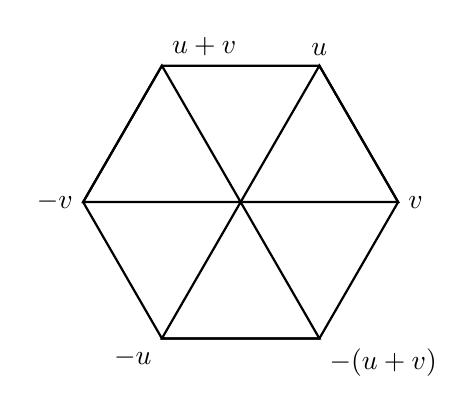
\begin{tikzpicture}[scale=2, thick]
% Define coordinates
\coordinate (O) at (0,0);
\coordinate (A) at (60:1);    % u
\coordinate (B) at (0:1);     % v
\coordinate (C) at (-60:1);   % -u
\coordinate (D) at (240:1);   % -(u+v)
\coordinate (E) at (180:1);   % -v
\coordinate (F) at (120:1);   % u+v

% Draw hexagon and diagonals
\draw (A)--(F)--(E)--(D)--(C)--(B)--cycle;
\draw (O)--(A)--(B)--(O);
\draw (O)--(C)--(D)--(O);
\draw (O)--(E)--(F)--(O);

% Labels
\node[above] at (A) {$u$};
\node[above right] at (F) {$u+v$};
\node[right] at (B) {$v$};
\node[left] at (E) {$-v$};
\node[below left] at (D) {$-u$};
\node[below right] at (C) {$-(u+v)$};
%\node at (O) {$O$};
\end{tikzpicture}
\end{center}
 Let $x =v$, $y = u+\dfrac{v}{2}$.Then it is evident that $x,y \in S_X$ and $x\perp_B y$.\\
 Now,
\[
\|x + y\| = \left\| v + \left( u + \tfrac{1}{2}v \right) \right\| 
= \left\| (u + v) + \tfrac{1}{2}v \right\| 
= \tfrac{3}{2} \left\| \tfrac{2}{3}(u + v) + \tfrac{1}{3}v \right\| 
= \tfrac{3}{2},
\]
and
\[
\|x - y\| = \left\| v - \left( u + \tfrac{1}{2}v \right) \right\| 
= \left\| -u + \tfrac{1}{2}v \right\| 
= \tfrac{3}{2} \left\| \tfrac{2}{3}(-u) + \tfrac{1}{3}v \right\| 
= \tfrac{3}{2}.
\]
\noindent Then it follows from the definition of $H_\nu(X,B)$ and the fact that 
$H_\nu(X,B)\leq \frac{3}{2}$ for any Radon plane that we derive
\[
\dfrac{3}{2}\geq H_\nu(X,B) \geq \frac{\|x+y\|^{\nu}\|x-y\|^{1-\nu} + \|x+y\|^{1-\nu}\|x-y\|^{\nu}}{2}=\dfrac{3}{2}.
\]
Therefore, $H_\nu(X,B)= \frac{3}{2}$.
This completes the proof.
\end{proof}


%% The Appendices part is started with the command \appendix;
%% appendix sections are then done as normal sections
%% \appendix

%% \section{}
%% \label{}

%% If you have bibdatabase file and want bibtex to generate the
%% bibitems, please use
%%
%%  \bibliographystyle{elsarticle-num} 
%%  \bibliography{<your bibdatabase>}

%% else use the following coding to input the bibitems directly in the
%% TeX file.

\begin{thebibliography}{00}

%% \bibitem{label}
%% Text of bibliographic item

\bibitem{birkhoff1935orthogonality}  G. Birkhoff, \textit{Orthogonality of matrices and some distance problems}. Duke Math. J. \textbf{1(2)}(1935), 169--172.

\bibitem{banas1986moduli}  J. Bana{\'s}, \textit{On moduli of smoothness of Banach spaces}. Bull. Pol. Acad. Sci. Math. \textbf{34(1)}(1986),  287–293.


\bibitem{baronti2000triangles}  M. Baronti, E. Casini, P. L. Papini, \textit{Triangles inscribed in a semicircle, in Minkowski planes, and in normed spaces}. J. Math. Anal. Appl.  \textbf{252(1)}(2000), 124--146.

%\bibitem{papini2022parameters} P. L. Papini and  M. Baronti, \textit{Parameters in Banach spaces and orthogonality}.  Constr. Math. Anal. \textbf{5(1)}(2022), 37--45.



\bibitem{clarkson1936uniformly} J. A. Clarkson, \textit{Uniformly convex spaces}. Trans. Amer. Math. Soc. \textbf{40(3)}(1936), 396--414.

\bibitem{james1964uniformly} R. C. Clarkson, \textit{Uniformly non-square Banach spaces}. Ann. Math. \textbf{80(3)}(1964), 542--550.

\bibitem{dinarvand2019heinz} M.  Dinarvand, \textit{Heinz means and triangles inscribed in a semicircle in Banach spaces}. Math. Inequal. Appl. \textbf{22(1)}(2019), 275--290.


\bibitem{du2023some} D. Du,  Y. Li, \textit{Some moduli and inequalities related to Birkhoff orthogonality in Banach spaces}. Aust. J. Math. Anal. Appl. \textbf{1}(2025), p.15.


\bibitem{du2025some} D. Du, R. Liang,  Y.Li, \textit{Some moduli of convexity and smoothness related to Birkhoff orthogonality in Banach spaces}. 	Rev. R. Acad. Cienc. Exactas Fís. Nat., Ser. A Mat. \textbf{119(4)}(2025), p.110.








%\bibitem{garcia2006uniformly} G. Falset, L. Fuster, M. Navarro, \textit{Uniformly nonsquare Banach spaces have the fixed point property for nonexpansive mappings}. J. Funct. Anal. \textbf{233(2)}(2006), 494--514.

\bibitem{fu2023relations} Y. Fu, Y. Li, \textit{The relations between the von Neumann--Jordan type constant and some geometric properties of Banach spaces}. Rev. Real Acad. Cienc. Exactas Fis. Nat. Ser. A-Mat. \textbf{117(1)}(2023), p. 25.

\bibitem{garcia2006uniformly} G. Falset, L. Fuster, M. Navarro, \textit{Uniformly nonsquare Banach spaces have the fixed point property for nonexpansive mappings}. J. Funct. Anal. \textbf{233(2)}(2006), 494--514.

\bibitem{gao1990geometry} J. Gao and K. Lau, \textit{On the geometry of spheres in normed linear spaces}. J. Aust. Math. Soc \textbf{48(1)}(1990), 101--112.

\bibitem{james1947orthogonality} R. C. James,
\textit{Orthogonality and linear functionals in normed linear spaces}. Trans. Amer. Math. Soc. \textbf{62(2)}(1947), 265--292.

\bibitem{james1947inner} R. C. James, \textit{Inner products in normed linear spaces}. Bull. Am. Math. Soc. \textbf{53(6)}(1997), 559--566.



\bibitem{joly1969caracterisations}  J. Joly, \textit{Caracterisations d'espaces hilbertiens au moyen de la constante rectangle}.  J. Approx. Theory \textbf{2(3)}(1969), 301--311.


\bibitem{papini2022parameters} P. L. Papini, M. Baront{\i}, \textit{Parameters in Banach spaces and orthogonality}. 	Constr. Math. Anal., \textbf{5(1)}(2022), 37--45.

\bibitem{pisier2016martingales} G. Pisier, \textit{Martingales in Banach spaces}. Cambridge University Press: Cambridge, UK, 2016; Volume 155, pp. 446–447.


\end{thebibliography}
\end{document}
\endinput
%%
%% End of file `elsarticle-template-num.tex'.
